\section{О стабилизации программных движений двузвенного манипулятора} \label{p23}
Рассмотрим решение задачи о стабилизации программного движения $(q_0 (t), \dot q_0 (t))$ в области 
$$G = {(x, \dot x) \in R^4 : \|x\|<\varepsilon, \quad \|\dot x\|<\varepsilon, \quad \varepsilon=const>0}$$
$$x = q - q_0 (t), \ \dot x = \dot q - \dot q_0 (t)$$
с помощью непрерывного управления вида
\begin{equation}
U^{(1)}(x, \dot x) = B(\dot x + p(x))
\end{equation}    
где $B \in R^{2 \times 2}$ есть матрица коэффициентов усиления сигналов, подлежащая определению.
Возьмем для системы (2.5) вектор-функцию Ляпунова $V = (V^1, V^2)^{'}$  с коэффициентами вида $$V^1 = \|p(x)\|, \quad V^2 = \sqrt{(\dot x + p(x))^{'} A^{(1)}(t, x)(\dot x + p(x)).}$$
Вычисляя производную по времени вектор-функции Ляпунова $V$ в силу системы (2.5), получим следующие оценки:
\begin{equation}
\begin{array}{l}
\dot V^1 \le -mu_1 V^1 + \frac{m_1}{\lambda_1},\\
\dot V^2 \le m_2 V^1 - \mu_2 V^2 + m_3 (V^1)^2 + m_4 (V^2)^2 + m_5 V^1 V^2, 
\end{array}
\end{equation}

где положительные постоянные $\mu_1, \mu_2, \lambda_1, m_i (i=1,2,...,5)$ определяются из следующих условий:
$$
\begin{array}{l}
\displaystyle \lambda_1^2 = \frac{I_1 + m_2 l_1^2 + I_2 - \sqrt{(I_1 + m_2 l_1^2 - I_2)^2} + 4(m_2 l_1 l_{g_2})^2}{2}\\
\displaystyle \lambda_2^2 = \frac{I_1 + m_2 l_1^2 + I_2 + \sqrt{(I_1 + m_2 l_1^2 - I_2)^2} + 4(m_2 l_1 l_{g_2})^2}{2}\\
\displaystyle \mu_1 =\frac12 \cos(\frac{\varepsilon}{2}), \quad m_1 = \frac12,\\
\displaystyle m_2 = \max \frac{\lambda_2^2 + 2 \sqrt{\lambda_{max} [(D-F)^{'} (D-F)]}}{2 \lambda_1},\\
\displaystyle m_3 = \frac{m_2 l_1 l_{g_2}}{\lambda_1}, \quad m_4 = \frac{2 m_2 l_1 l_{g_2}}{\lambda_1}, \quad m_5 = \frac{3 m_2 l_1 l_{g_2}}{\lambda_1},\\
\displaystyle \mu_2 = \frac{-\lambda_2^2 - 4 g_1 m_2 l_q l_{g_2} - \lambda_{max} (B + B^{'})}{2 \lambda_2}
\end{array}
$$

Здесь $\lambda_{max}$ есть максимальное собственное значение соответствующей матрицы. 
Тогда для системы (2.9) можно построить следующую систему сравнения:

\begin{equation}\label{2.4'}
\dot u^1 = - \mu_1 u^1 + \frac{m_1}{\lambda_1} u^2, \quad \dot u^2 = m_2 u^1 - \mu_2 u^2 + m_3 (u^1)^2 + m_4(u^2)^2 + m_5 u^1 u^2
\end{equation}

Согласно теореме сравнения об асимптотической устойчивости \cite{matrosov01} из свойства асимптотической устойчивости нулевого решения системы сравнения (2.13) следует свойство равномерной асимптотической устойчивости нулевого решения системы (2.2). Получим условие асимптотической устойчивости нулевого решения системы (2.13) с областью притяжения $$ {(u^1, u^2) \in R^2 : 0 \le u^1 \le \delta_1 = const>0, 0 \le u^2 \le \delta_2 = const>0}. $$ Пусть найдется такое число $\gamma>0$, что выполняются соотношения:

\begin{equation}\label{2.10'}
\gamma = \frac{\delta_2 m_1}{\delta_1 \lambda_1 \mu_1}, \quad \mu_2 > \frac{m_1}{\gamma \lambda_1 \mu_1} (m_2 + \delta_1 m_3) + m_4 \delta_2 + m_5 \delta_1
\end{equation}

Тогда можно показать, что функция $\widetilde{u}(t) = \max{(u^1(t), \delta_1 u^2(t)/ \delta_2)}$ будет монотонно стремиться к нулю при $t \to \infty$, и, значит, нулевое решение системы сравнения (2.13) будет асимптотически устойчиво.
При невозможности практической реализации программного управления (2.3) и (2.4) стабилизацию программного движения можно осуществить[] при помощи релейного управления вида

\begin{equation} \label{2.11'}
U^{(1)}(x, \dot x) = B \ sign(\dot x + p(x))
\end{equation}

Численное моделирование управляемого движения манипулятора проводилось при следующих значениях параметров манипулятора и программной траектории:
$$q_1^0(t) = \sin(0,5t), \quad q_1^0(t) = \cos(0,5t) + \pi/2$$

На рисунках 2.6 и 2.6 представлены результаты моделирования при управлениях (2.11) и (2.15) соответственно при начальных значениях $q_{10} = 0.5, \dot q_10 = -0.5, q_{20} = 2.1, \dot q_{20} = 0.3$ 

Стоит отметить, что при использовании непрерывного управления (2.11) использовалась матрица коэффициентов в виде $B=35E$ , где $E$  --- единичная матрица. А при использовании релейного закона (2.15) сократились энергозатраты на управление, так как матрица коэффициентов усиления была найдена в виде $B = diag \lbrace 5, 2 \rbrace.$ 

\begin{figure}[h]
 	\centering
 	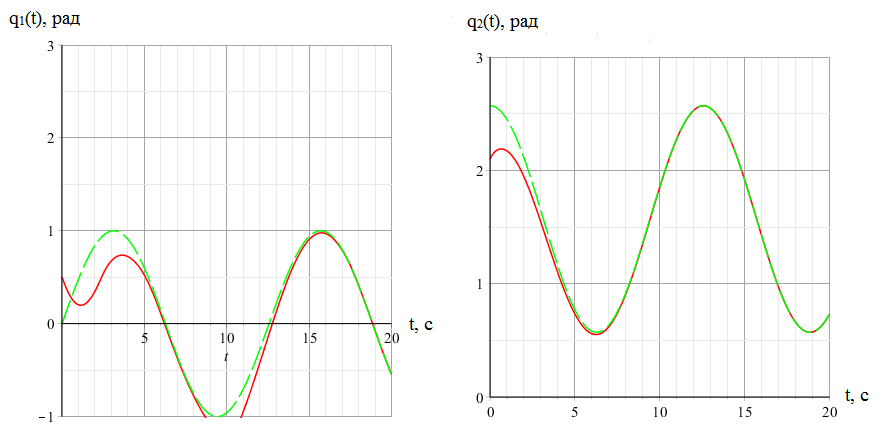
\includegraphics[width=1.0\textwidth]{signum}
 	\caption{Результаты моделирования при управлении (2.11)}
\end{figure}

\begin{figure}[h]
	\centering
	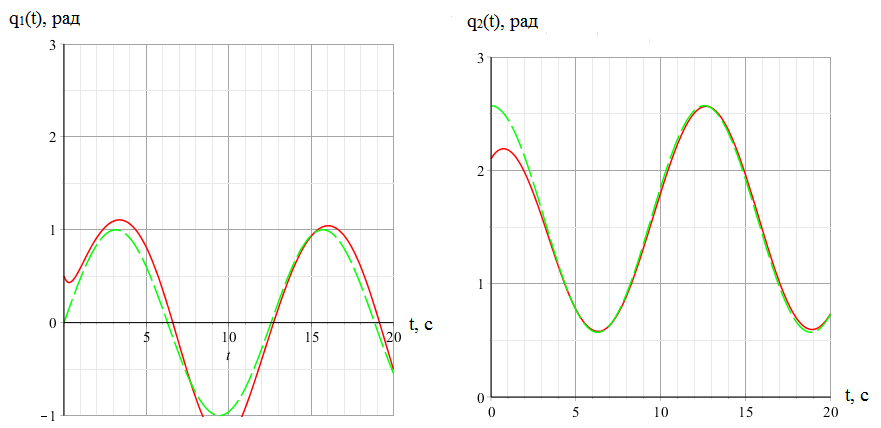
\includegraphics[width=1.0\textwidth]{without_signum}
	\caption{Результаты моделирования при управлении (2.15)}
\end{figure}
